\documentclass{whutmod}
\usepackage{metalogo}
\usepackage{float}
\usepackage{subfigure} 
\usepackage{url}
\usepackage{setspace}
\usepackage{booktabs}
\bibliographystyle{unsrt}
\team{23}
\membera{刘子川}
\joba{编程}
\memberb{程宇}
\jobb{建模}
\memberc{祁成}
\jobc{建模}
\hypersetup{
	colorlinks=true,
	linkcolor=black
}
\newcommand{\upcite}[1]{\textsuperscript{\cite{#1}}}
\title{基于xx模型}
\tihao{1} 

\begin{document}

%\maketitle

	%目录
	\thispagestyle{empty}
	\tableofcontents
	\setcounter{page}{0}                                               
	\newpage	%换页符
	

	
	\section{问题重述}	
	\subsection{问题背景}
   在物资调运过程中,完成指定点的调运任务是最基本
   的要求,在完成基本的任务之外,往往有更高的追求,比如
   如何使总运费最省?怎样才能使得运输时间最短?如何选
   择运输路径使得运输总距离最短等等。这些更高的追求往
   往是企业期望达到的目标,为了解决这些类似问题,有必
   要对物资调运的过程进行数学模型的建立,以期通过模型
   来理解和分析物资调运的过程,并为其找到解决的方法。
   现以具体的食品调运案例进行分析研究\upcite{bib:one}。
    
    某食品公司有19个食品销售点,销售点的地理坐标和每天的需求量见附件。每天凌晨都要从仓库(第20号站点)出发将食品运至每个销售点,运送物品后最终返回仓库。现有运送食品的运输车,每台车每日工作 4小时,运输车重载运费2元/吨公里,并且假定街道方向均平行于坐标轴,任意两站点间都可以通过一次拐弯到达。

	\subsection{问题概述}
    围绕相关附件和条件要求,研究食品运输车在各仓库间的调度方案,依次提出以下问题:
		 
	
	\textbf{问题一:}若只有一辆载重100吨的大型运输车,运输车平均速度为40公里/小时,每个销售点需要用20分钟的时间下货,空载费用0.6元/公里。它送完所有食品并回到仓库,求最少需要时间及其对应的总距离,总运费。
	
	\textbf{问题二:}有一种小型运输车,运输车平均速度为50公里/小时,每个销售点需要用5分钟的时间下货,载重为6吨,空载费用0.4元/公里;要使它们送完所有食品并回到仓库,运输车应如何调度使总体调度效率最高? 
	
	\textbf{问题三:}如果有载重量为4吨、6吨两种运输车,空载费用分别为0.2、0.4元/公里,其他条件均相同,又如何安排车辆数和调度方案。

	
	\section{模型假设}
	
	\begin{itemize}                                             
		\item [(1)] 假设汽车速度均匀,不会随载重而发生变化。
		\item [(2)] 假定街道方向均平行于坐标轴,任意两站点间都可以通过一次拐弯到达。
	\end{itemize}
		
	\section{符号说明}
	\begin{table}[H]
	\label{biao} \centering
	\begin{tabular}{cc}
		\toprule[1.5pt]
		\multicolumn{1}{m{5cm}}{\centering 符号} & \multicolumn{1}{m{5cm}}{\centering 说明} \\
		\midrule[0.5pt]		
		$P_n$  & 20个站点  \\ 
		$d$  &  曼哈顿距离 \\ 
		$f$  &  最短路径\\
		$\left \{ A_n \right \}$  &  原始染色解集\\
				$W(B_k)$  & 小车k的总重量和\\
						$T(B_k)$  & 货运总时间\\
		$\Gamma (P_n)$  & 运输成本目标函数\\
		$B_k$  & k量小型运输车路径\\
		$\theta$&惩罚因子\\
		\bottomrule[1.5pt]
	\end{tabular}
\end{table}

	\section{问题一模型的建立与求解}
    \subsection{问题描述与分析}
问题一要求规划大型运输车的行驶路径,使得货物运输时间达到最短。该问题本质是旅行商问题,基于街道方向均平行于坐标轴,我们求解任意两点间的曼哈顿距离作为其间的距离,并设计动态赌轮遗传算法对其进行求解。


    其思维流程图如图~\ref{lct}~所示:

       \begin{figure}[H]
	   	\centering
	   	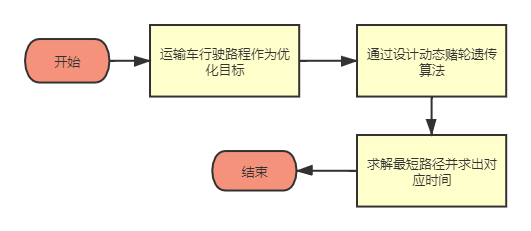
\includegraphics[width=\textwidth]{figures/abab.png}
	   	\caption{问题一思维流程图}\label{lct}
	   \end{figure}

   
	    \subsection{模型的建立}
	    \subsubsection{经典旅行商模型}
	    分析问题一,由于大型运输车的行驶速度固定,优化行驶路径使得运输车行驶路程最短时,即可求得最小运输时间。遍历路径可表示为二维有限序列如下:
	     \begin{gather}
	    P_n=[p_{1},p_{2},\cdots,p_{i},\cdots,p_{19}] ,
	    \end{gather}
	    其中$p_{i}(1\leqslant i \leqslant 19 ,i\in Z)$表示处运输起点外的的仓库坐标,且对于$\forall i \neq j$都有$p_i \neq p_j $。任意两坐标点$p_i(x_i,y_i)$,$p_j(x_j,y_j)$间的曼哈顿距离可表示为:
	     \begin{gather*}
	     d(p_i,p_j)=\left | x_i-x_j \right |+\left | y_i-y_j \right | ,
	     \end{gather*}
	     
	    将运输车行驶路程作为优化目标即可得到目标函数如下:
	    \begin{gather*}
	    f(P_n)=d(p_0,p_{1})+d(p_0,p_{19})+\sum_{i=1}^{18}d(p_i,p_{i+1}) ,
	    \end{gather*}
	    
	    即可得到整体优化模型如下:
	    \begin{gather}
	    f(P_n)=d(p_0,p_{1})+d(p_0,p_{19})+\sum_{i=1}^{18}d(p_i,p_{i+1}) ,\\
	    \left\{\begin{matrix}1\leqslant i \leqslant 19 ,i\in Z
	    \\ \forall i \neq j,p_i \neq p_j 
	    \end{matrix}\right.
        \end{gather}
        
        \subsection{模型的求解}
        \subsubsection{遗传算法}
        \paragraph{初始化编码}
        对于表示为二维有限序列的遍历路径$P_n$,对其进行整数编码为
        \begin{gather*}
        A_n=[a_{n1},a_{n2},\cdots,a_{ni},\cdots,a_{n19}], \\
        1\leqslant a_i \leqslant 19 ,i\in Z ;\forall i, \neq j\Rightarrow p_i \neq p_j 
        \end{gather*}
        
        定义$A_n$为解序列$P_{n}$,其中$a_{ni}$表式对应仓库的访问顺序,例如 $a{i}=7$表示第$i$次访问7号仓库。即随机生成初始解集$A=\left \{A_n\right \}$其中$n=1,2,\cdots,w$, w为的种群容量。
        
        \paragraph{交叉}
        在原染色解集 $\left \{ A_n \right \}$中的染色体按照随机顺序配对,按照以下的方式交叉(补全),生成交叉解集$\left \{H_n\right \}$,为保证变异率并保留优秀基因片段和本题采用的两种交叉方式:
        
        \begin{itemize}
        	\item [(1)]单点交叉:
        	
        	对于两个父代个体$ A_n=[a_{n1},a_{n2},\cdots,a_{ni},\cdots,a_{n19}]$和$H_n=[a_{n1}',a_{n2}',\cdots,a_{ni}',\cdots,a_{n19}']$,随机选择第$k$个基因处为交叉点,将该基因后所有基因进行交换,得到子代基因。
        	\item [(2)]中间值交叉:
        	
        	对于两个父代个体$ A_n=[a_{n1},a_{n2},\cdots,a_{ni},\cdots,a_{n19}]$和	$H_n=[a_{n1}',a_{n2}',\cdots,a_{ni}',\cdots,a_{n19}']$,随机选取$a_{k}''\in [a_{k},a_{k}']$得到子代基因。
        \end{itemize}
        再选取交叉个体时采用混合分组的方法,将父代均匀混合后选取所有编号为奇数的个体,与其相邻对应编号为偶数的个体,通过两种交叉方式产生处两种类型的子代。
    	其过程如下表所示:
    	  	\begin{table}[H]
    		\centering	
    		  		\setstretch{1.5}  %设置表的行间距
    		  			\caption{各个小型运输车对应运输路径方案}\label{zhuansasgggggzai}
    		\begin{tabular}{cc}
    			\toprule[2pt]
    			\multicolumn{1}{m{3cm}}{\centering 交叉片段编号}
    			& \multicolumn{1}{m{8cm}}{\centering 对应运输路线}
    			\\
    			\midrule[1pt]
    			基因序列$A_1$ &  [1,	2,	3,	4,	5,	6,	7,	8,	9,	10,	11,	12,	13,	14,	15,	16,	17,	18,	19] \\ 
    			基因序列$A_2$ &  [13,	11,	12,	19,	14,	15,	18,	16,	17,	10,	9,	1,	2,	5,	6,	7,	4,	3,	8] \\ 
    			基因序列$A_3$ &  [13,	19,	12,	11	,6	,7,	5,	2	,4	,1	,3	,8	,9,	10,	17,	16,	18	,15,	14] \\ 
    			$\cdots$ & [$\cdots, \cdots, \cdots, \cdots$] \\ 
    			基因序列$A_{19}$ &  [20,8,3,4,5,2,1,9,10,17,16,18,14,15,19,13,11,12,6,7,20]\\ 
    			基因序列$A_{20}$ &  [20,8,3,4,5,2,1,9,10,17,16,18,15,14,19,13,12,11,6,7,20] \\ 
    			\bottomrule[2pt]	
    		\end{tabular}
    	\end{table}
    	
    	
         \paragraph{变异}
         鉴于序列式染色体的特殊性,为了在变异阶段内尽可能不破坏原有的基因段,采取改良圈算法的思路进行变异操作。即在染色体$A$中随机选取$a_{i}$与$a_{j}(1\leqslant i<j\leqslant j )$,颠倒$a_{ni}$与$a_{nj}$间顺序的顺序,即:
          \begin{gather}
          M=[a_{1},\cdots,a_{i},a_{j-1},a_{j-2},\cdots,a_{i+1},a_{i},\cdots,a_{19}]
          \end{gather}
          $M$为染色体$A$对应的变异染色体,对于每个染色体$A_n$,都设定相同的变异概率$\gamma$去执行上述的变异操作。 
         \subsubsection{动态赌轮}
         将第g代的染色体与其交叉和变异产生的子代并入同一解集$G_g=\left \{A,H,M\right \}$。$k$表示原解集$A$,交叉解集$H$和变异解集$M$中解的数量之和,即为$G_g$中的解的数目。设置$G_g$第$i$个解$G_g(i)$被选择进入下一代的概率为:
         \begin{gather}
          P(G_{g}(i))=\frac{wf^{-g/\gamma }(G_{g}(i))}{\sum_{j=1}^{k}f^{-g/\gamma }(G_{g}(j))},
         \end{gather}
         $f^{-g/\gamma }(G_{g}(i))$为$G_{g}(i)$对应的目标函数值,即为$G_{g}(i)$对应的适应度。其中参数$\gamma$为衰减系数,$w$为种群容量。即适应度值相对较小的解保留概率将逐渐增大,
         即算法初始阶段将保留丰富度尽可能多的解,而愈到算法后期,策略就越接近于精英策略,加快算法的收敛速度,即有:
           \begin{gather}
           \lim_{g\rightarrow \infty } P(G_{g}(min))=\lim_{g\rightarrow \infty }\frac{wf^{-g/\gamma }(min)}{\sum_{j=1}^{k}f^{-g/\gamma }(G_{g}(j))}\rightarrow 1 ,
         \end{gather}
         该式表明当迭代次数$g$足够大时,选择策略将趋近于为精英策略,将加速算法的收敛。重复上述进化过程,当进化代数足够多时,求解得到全局最优解。
         
         
      \subsection{实验结果及分析}
      遗传算法的算法收敛图如图\ref{llsffssl}所示:
               \begin{figure}[H]
      	\centering
      	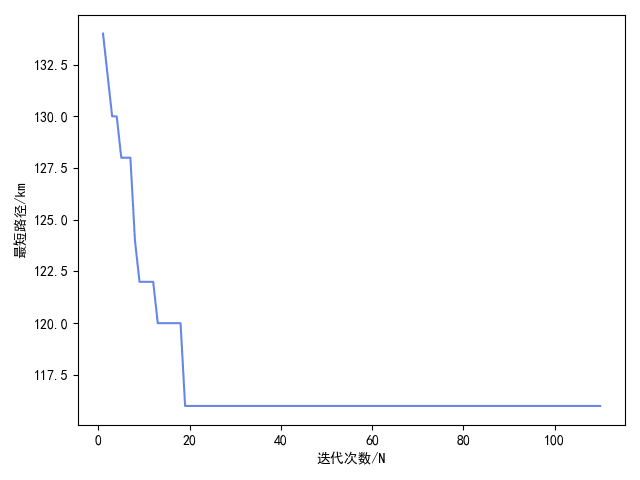
\includegraphics[width=\textwidth]{figures/y1.png}
      	\caption{遗传算法收敛图
      	}\label{llsffssl}
      \end{figure}
      
      
      
      由算法收敛图可知算法收敛速度较快,早熟问题解决的较好,全局搜素能力较强, 求得最短距离为116km,其最优个体基因为:
               \begin{gather*}
      route = [20,8,3,4,5,2,1,9,10,17,16,18,15,14,19,13,12,11,6,7,20].
      \end{gather*}

      
      其对应大型运输车运输方案为route的路径如图 \ref{llsssl}所示:
  
         \begin{figure}[H]
         	\centering
         	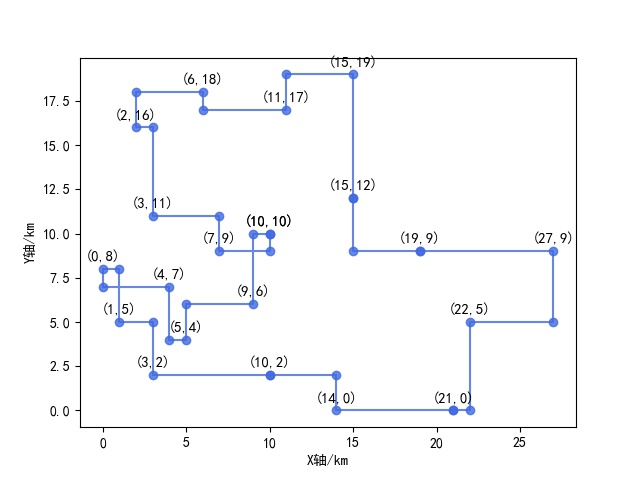
\includegraphics[width=\textwidth]{figures/11.jpg}
         	\caption{大型运输车运输方案路径}\label{llsssl}
         \end{figure}
     
     则大型送完所有食品并回到仓库,最少需要2.9时间,总费用为7695.2元。
     
 \section{问题二模型的建立与求解}
 
\subsection{问题描述与分析}
问题二要求设计小型运输车的调度方案,从而使得总体调度效率最高。我们将时间限制设置为约束,着重优化方案的经济效率。在问题一的基础上重新建立模型,鉴于第二问的决策变量是多段序列的和,我们设计了插板编码对决策变量进行编码,并基于问题一中的动态赌轮遗传算法以运输总成本为目标进行优化。

    其思维流程图如图~\ref{lssssct}~所示:

\begin{figure}[H]
	\centering
	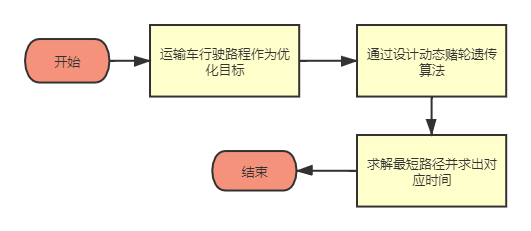
\includegraphics[width=\textwidth]{figures/abab.png}
	\caption{问题二思维流程图}\label{lssssct}
\end{figure}

\subsection{带约束的多旅行商模型}
当雇佣$b$辆小型运输车时,总决策序列可表示为
\begin{gather*}
P_n=\left \{[p_{1},p_{2}]_1,[\cdots,p_{i}]_k,[\cdots]_{b-1},[p_{19}]_b\right \},
\end{gather*}

即将类似于模型一中的坐标序列分割为多段,每一段分别由一辆小型运输车单独完成,定义小型运输车$k$的运输路径为:
\begin{gather*}
B_k=[p_{i},p_{i+1},\cdots,p_{j-1},p_{j}]_k,
\end{gather*}
即总路径决策变量可表示为:
\begin{gather*}
P_n=\left \{B_1,B_2,\cdots,B_b\right \}.
\end{gather*}

小车$k$的载重总和可表示为:
\begin{gather}
W (B_k)=\sum_{p_i\in B_k}w(p_{i}),
\end{gather}

其中$w(p_{i})$为仓库$p_{i}$的订货量。其货运总时间可表示为:
\begin{gather}
T (B_k)=L(B_k)/50+size(B_k)/12,
\end{gather}

将运输成本作为目标函数可表示为:
\begin{gather*}
\Gamma (P_n)=\sum _{k=1}^b[\sum _{j=1}^{size(B_k))}(0.4+2\sum _{i=1}^jw(p_i))\times d(p_i,p_{i+1})_{pi\in B_k}].
\end{gather*}

小型运输车的负载量约束可表示为:
\begin{gather*}
\underset{B_k\in P_n}{max}  W (B_k) \leqslant 6,
\end{gather*}

其运输时间约束可表示为时间约束可表示为:
\begin{gather*}
\underset{B_k\in P_n}{max}  T (B_k) \leqslant 4,
\end{gather*}
即整体模型可以表示为
\begin{gather}
\Gamma (P_n)=\sum _{k=1}^b[\sum _{j=1}^{size(B_k))}(0.4+2\sum _{i=1}^jw(p_i))\times d(p_i,p_{i+1})_{pi\in B_k}]\\
\left\{\begin{matrix}\underset{B_k\in P_n}{max}  W (B_k) \leqslant 6
\\ \underset{B_k\in P_n}{max}  T (B_k) \leqslant 4
\end{matrix}\right.
\end{gather}
\subsection{模型的求解}
\subsubsection{插板式编码遗传算法}
由于问题中的决策变量$P_n$表示多个不同小型运输车的运输路径,我们将染色体变量中插入无意义基因作为隔板,例如在派遣两辆运输车时,决策变量可表示为
\begin{gather*}
P_n=\left \{[p_{1},p_{2},\cdots,p_{i}]_1,[p_{i+1}\cdots,p_{19}]_{2}\right \},
\end{gather*}

即在染色体中插入一个无意义基因作为挡板即可表示出染色体:
\begin{gather*}
A_n=[a_{n1},a_{n2},\cdots,a_{ni},\varphi ,a_{ni+1},\cdots,a_{n19}].
\end{gather*}

其中$\varphi$为无意义挡板基因。当雇佣小型运输车数量为$N$时,在染色体中插入$N-1$个挡板基因即可将染色体分成$N$段,即能分别代表每辆小车的行驶的路径。之后将无意义挡板基因作为普通基因进行交叉,变异即可优化求解每一辆小车的行驶路径。引入冗余惩罚因子$\theta$ :
\begin{gather}
\theta(P_n)=\left\{\begin{matrix}1,(\exists (Loc(\varphi_i )+1)=Loc(\varphi_{i+1} ))\vee  (\exists (Loc(\varphi_i )=0)\vee (\exists (Loc(\varphi_i )=size(A_n))
\\ 0,otherwise
\end{matrix}\right.
\end{gather}

其中$Loc(\varphi_i )$表示无意义挡板基因$\varphi_i$在染色体$A_n$中的位置,$size(A_n)$表示染色体$A_n$的维数。即当决策变量$P_n$中的挡板基因存在于其开头或末尾时,或者当两个挡板基因相邻时,表明有被雇佣车辆并没有参加运输工作,此时将惩罚因子$\theta(P_n)$置一,否决置零。

求解第二问时,我们沿用第一问的动态赌轮遗传算法进行优化计算。即将目标函数替换为:
\begin{gather}
F(P_n)= \Gamma (P_n)+\theta(P_n)M_1+max(\underset{B_k\in P_n}{max} W (B_k)-6 ,0) M_2+max(\underset{B_k\in P_n}{max}T (B_k)-4,0)M_3
\end{gather}
其中$M_1$、$M_2$和$M_3$为较大的正系数,即可达到罚函数约束功能。
 
  
        \subsection{实验结果及分析}
%  遗传算法的算法收敛图如图 ????所示:
%  
%  909.800000000000	852.600000000000	850.000000000000	815.300000000000	800.700000000000	842.600000000000	810.000000000000	856.200000000000
实验从六量车到十三量车每个模型计算了100次迭代之后,其各自费用为:

  	\begin{table}[H]
	  		\setstretch{1.5}  %设置表的行间距
	\centering		
	\caption{每组小型运输车对应运输路径总费用}\label{zhuanssssasgzai}
	\begin{tabular}{cc}
		\toprule[2pt]
		\multicolumn{1}{m{5cm}}{\centering 运输车数量}
		& \multicolumn{1}{m{5cm}}{\centering 对应运输路径总费用}
		\\
		\midrule[1pt]
		6量运输车 &   909.80\\ 
		7量运输车 & 	852.60\\ 
		8量运输车 &  	850.00 \\ 
		9量运输车 &  815.30 \\ 
		10量运输车 &   800.70\\ 
	11量运输车 & 	842.60 \\ 
		12量运输车 &810.00\\ 
		13量运输车 & 	856.20\\ 
		\bottomrule[2pt]	
	\end{tabular}
\end{table}
  
  由表\ref{zhuanssssasgzai}可知求得所需要10量小型运输车时,调运方案所需要的运输费用最小,并给出最优个体基因如表\ref{zhuansassgzai}所示:%为$routes = [[0, 14, 0], [0, 18, 15, 0], [0, 10, 9, 0], [0, 17, 16, 0], [0, 12, 11, 0], [0, 4, 2, 3, 8, 0], [0, 5, 1, 0], [0, 19, 0], [0, 6, 7, 0], [0, 13, 0]]$。
  
  	\begin{table}[H]

  	\centering		
  	\caption{各个小型运输车对应运输路径方案}\label{zhuansassgzai}
  		\setstretch{1.5}  %设置表的行间距
  	\begin{tabular}{cc}
  		\toprule[2pt]
  		\multicolumn{1}{m{5cm}}{\centering 运输车编号}
  		& \multicolumn{1}{m{5cm}}{\centering 对应运输路线}
  		\\
  		\midrule[1pt]
  		1号运输车 &  [20, 14, 20] \\ 
  		2号运输车 &  [20, 18, 15, 20] \\ 
  		3号运输车 &  [20, 10, 9, 20] \\ 
  		4号运输车 &  [20, 17, 16, 20] \\ 
  		5号运输车 &   [20, 12, 11, 20]\\ 
  		6号运输车 & [20, 4, 2, 3, 8, 20] \\ 
  		7号运输车 & [20, 5, 1, 20] \\ 
  		8号运输车 &  [20, 19, 20] \\ 
  		9号运输车 &   [20, 6, 7, 20] \\ 
  		10号运输车 & [20, 13, 20] \\
  		\bottomrule[2pt]	
  	\end{tabular}
  \end{table}
  
  其对应各量小型运输车运输方案为routes的路径如图 \ref{ssssssss}所示,每一辆运输车的对应运输均用两点间哈曼吨距离表示,其中箭头表述运输的方向,得到10量小型运输车的运输方案路径图如下:
  
  \begin{figure}[H]
  	\centering
  	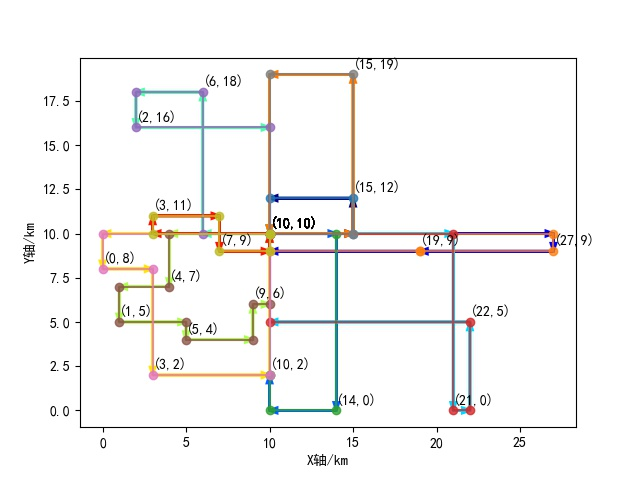
\includegraphics[width=\textwidth]{figures/22.jpg}
  	\caption{小型运输车运输方案图}\label{ssssssss}
  \end{figure}

其各个小车的运输细节图下图所示:
\begin{figure}[H]
	\centering
	\subfigure{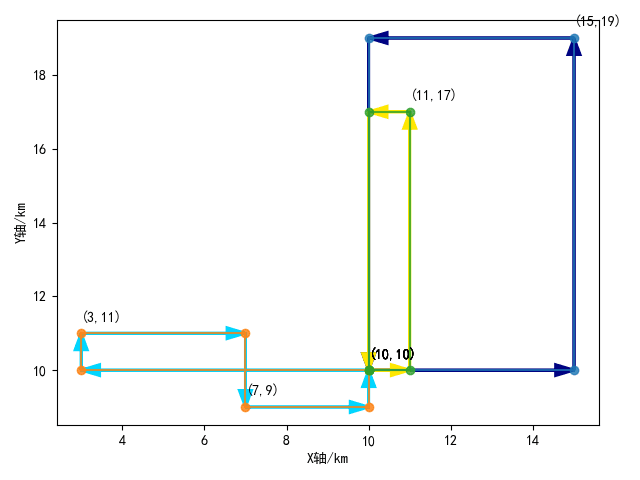
\includegraphics[height=8cm,width=7.5cm]{figures/1.png}}
	\subfigure{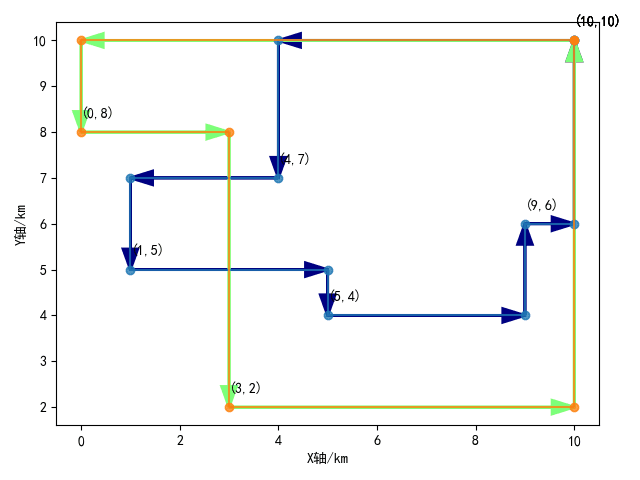
\includegraphics[height=8cm,width=7.5cm]{figures/2.png}}
\end{figure}	
\begin{figure}[H]	
	\centering
	\subfigure{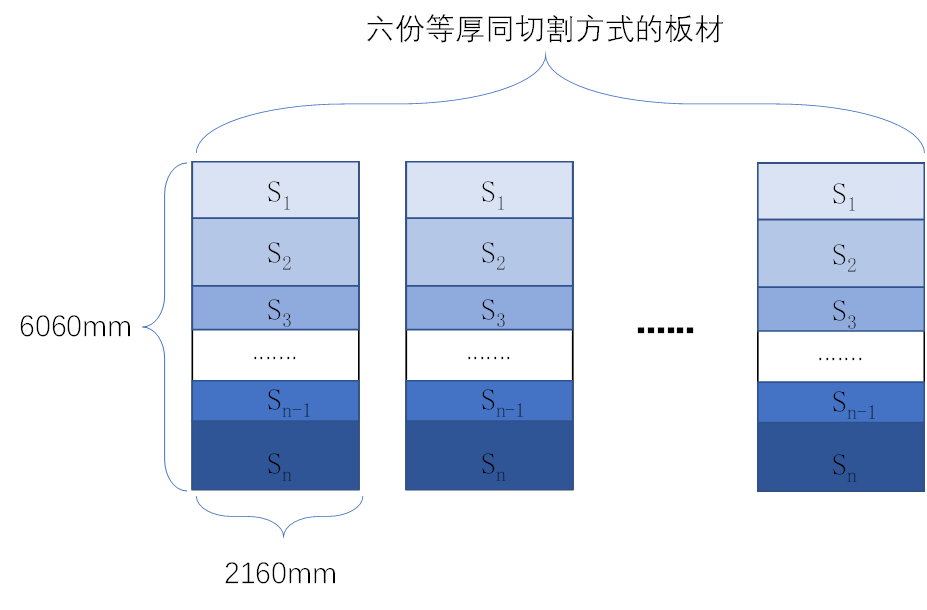
\includegraphics[height=8cm,width=7.5cm]{figures/3.png}}
	\subfigure{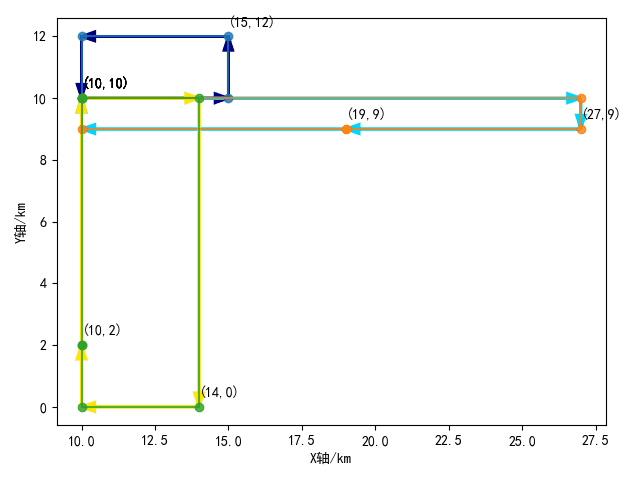
\includegraphics[height=8cm,width=7.5cm]{figures/4.png}}
	\caption{各个小车的运输细节图}
	\label{fisg}
\end{figure}

    \section{问题三模型的建立与求解}
  针对第三问,我们在第二问模型的基础上,引入启发式算法以决策每个任务需要派遣何种类型的小车。首先沿用第二问模型的插板式编码方法,在适应度计算时分析每个小车的负载情况,并由此作为依据派遣小车。再通过交叉,变异及动态赌轮选择操作,优化出最合理的小车调度方案。  
  \subsection{模型的求解}
  \subsubsection{启发式调度算法}
  在计算总运费时,针对运输车$k$的任务$B_k$,使得:
  \begin{gather}
  \alpha (B_k)=\left\{\begin{matrix}0.2,0<W(B_k)\leqslant4
  \\ 0.4,4<W(B_k)\leqslant6
  \end{matrix}\right.
  \end{gather}
  其中$\alpha (B_k)$为任务$B_k$中的空载运输费用。即将成本目标函数修改为:
  \begin{gather}
  \Gamma '(P_n)=\sum _{k=1}^b[\sum _{j=1}^{size(B_k))}(\alpha (B_k)+2\sum _{i=1}^jw(p_i))\times d(p_i,p_{i+1})_{pi\in B_k}]
  \end{gather}
  其对应的优化目标函数可表示为:
  \begin{gather}
  F(P_n)'= \Gamma '(P_n)+\theta(P_n)M_1+\sum_{B_k\in P_n}max( W (B_k)-6 ,0) M_2+max(\underset{B_k\in P_n}{max}T (B_k)-4,0)M_3
  \end{gather}
  以  $F(P_n)'$为目标函数进行动态赌轮遗传算法即可得到最终的最优调度方案。
  \subsection{结果分析}
  
  
%  \section{灵敏度分析}
  
  
  
  \section{模型的评价}
  \subsection{模型的优点}
  \begin{itemize}                                             
  	\item [(1)] 使用遗传算法,具有很强的全局搜索能力和鲁棒性,运算时间远小于全遍历算法。
  	
  	\item [(2)] 针对支持向量回归参数选取,利用灰色关联度筛选合适指标,相较于主观选取指标具有客观性、严谨性。	
  \end{itemize}
  \subsection{模型的缺点}
  
多目标遗传算法初始解由卡特蒙洛法随机生成,每次搜索结果不完全相同,可能引起结果 的偏差,需要多搜索几次选择才能得到最优结果。

  \subsection{模型改进}
  
可使用改进的生命遗传算法,加强算法的局部搜索能力,解决算法早熟的问题。

  
  
  
 
	\newpage	%换页符
	%%参考文献
	%\begin{thebibliography}{9}%宽度9
	% \setlength{\itemsep}{-2mm}
	\nocite{*}		%排版未引用的参考文献
%\bibliography{wenxian.bib}
%	%参考文献添加到wenxian.bib里,再引用
%	
\begin{thebibliography}{9}%宽度9
	\bibitem{bib:one}张斯嘉, 郭建胜, 钟夫, 等. 基于蝙蝠算法的多目标战备物资调运决策优化[J]. 火力与指挥控制, 2016, 41(1): 58-61.
	\bibitem{bib:2}李健, 张文文, 白晓昀, 等. 基于系统动力学的应急物资调运速度影响因素研究[J]. 系统工程理论与实践, 2015, 35(3): 661-670.	
	\bibitem{3}Wang J, Ersoy O K, He M, et al. Multi-offspring genetic algorithm and its application to the traveling salesman problem[J]. Applied Soft Computing, 2016, 43: 415-423.
	\bibitem{4}陶丽华, 马振楠, 史朋涛, 等. 基于 TSP 问题的动态蚁群遗传算法[J]. 机械设计与制造, 2019 (12): 39.
\end{thebibliography}

	\newpage
	%附录
	\appendix %%附录

\section{模型的代码实现}

\subsection{GATSP--matlab源代码}
\begin{lstlisting}[language=matlab]
clear;
w=20;g=100;d=19;%w为种群数,g代数,d维数
G(1:w,1:d)=0;%初始化空间
for i=1:w%初始化
c=randperm(d);
for t=1:20
flag=0;
for t1=1:d-1
for t2=t1+1:d
cl=c;
cl(t1:t2)=cl(t2:-1:t1);
if distan(cl)<distan(c)
c=cl;
flag=1;
end
end
end
if flag==0
G(i,1:d)=c;break
end
end
end
for k=1:g %进入遗传循环
A=G;%预备交叉阵
c=randperm(w);%配对序列
%c=1:w;
for i=1:2:w %交叉
F1=ceil(rand*d);%交叉点1
F2=ceil(rand*d);%交叉点2
while(F1==F2)
F2=ceil(rand*d);
end
if(F1>F2)%交叉地址调序
tem=F1;
F1=F2;
F2=tem;
end
j=0;t=1;%计数标值
while(j~=d+F1-F2-1)%如果剩余基因没完全插入就继续
if(isempty(find(A(c(i),F1:F2)==G(c(i+1),t),1))) %目标基因于交换片段中都不同
j=j+1;
if j<F1 %前半段基因交换
A(c(i),j)=G(c(i+1),t);
A(c(i+1),t)= G(c(i),j);
else %后半段基因交换
A(c(i),j+F2-F1+1)=G(c(i+1),t);
A(c(i+1),t)=G(c(i),j+F2-F1+1);
end
end
t=t+1;
end
end
by=[];
while isempty(by)
by=find(rand(1,w)<0.3);%变异地址
end
B=G(by,1:d);%预备变异阵
for j=1:length(by)
bw=sort(ceil(rand(1,2)*d));%变异基因节点
B(j,bw(1))=G(j,bw(2));%单点基因交换
B(j,bw(2))=G(j,bw(1));
end
GG=[G;A;B];%GG为选择阵    
clear A; clear B;%清除数据防止规格保存
m=size(G,1);%选择阵个体数
long(1:m)=0;%目标函数初始化
for i=1:m%计算函数
long(i)=distan(GG(i,:));
end
[slong,ind]=sort(long(1:m));%目标函数排序
for i=1:w%精英选择
G(i,:)=GG(ind(i),:);
end
clear GG;%清除数据防止规格保存
end      
\end{lstlisting}


\subsection{MGATSP--matlab源代码}
\begin{lstlisting}[language=matlab]
clear;
for pp=6:13 %6:13
for ppp=1:100
n=pp;w=20;g=100;d=19+n-1;%n为车数,w为种群数,g代数,d维数
G(1:w,1:d)=0;%初始化空间
for i=1:w%初始化
c=randperm(d);
for t=1:20
flag=0;
for t1=1:d-1
for t2=t1+1:d
cl=c;
cl(t1:t2)=cl(t2:-1:t1);
if price(cl)<price(c)
c=cl;
flag=1;
end
end
end
if flag==0
G(i,1:d)=c;break
end
end
end
for k=1:g %进入遗传循环
A=G;%预备交叉阵
c=randperm(w);%配对序列
%c=1:w;
for i=1:2:w %交叉
F1=ceil(rand*d);%交叉点1
F2=ceil(rand*d);%交叉点2
while(F1==F2)
F2=ceil(rand*d);
end
if(F1>F2)%交叉地址调序
tem=F1;
F1=F2;
F2=tem;
end
j=0;t=1;%计数标值
while(j~=d+F1-F2-1)%如果剩余基因没完全插入就继续
if(isempty(find(A(c(i),F1:F2)==G(c(i+1),t),1))) %目标基因于交换片段中都不同
j=j+1;
if j<F1 %前半段基因交换
A(c(i),j)=G(c(i+1),t);
A(c(i+1),t)= G(c(i),j);
else %后半段基因交换
A(c(i),j+F2-F1+1)=G(c(i+1),t);
A(c(i+1),t)=G(c(i),j+F2-F1+1);
end
end
t=t+1;
end
end
by=[];
while isempty(by)
by=find(rand(1,w)<0.3);%变异地址
end
B=G(by,1:d);%预备变异阵
for j=1:length(by)
bw=sort(ceil(rand(1,2)*d));%变异基因节点
B(j,bw(1))=G(j,bw(2));%单点基因交换
B(j,bw(2))=G(j,bw(1));
end
GG=[G;A;B];%GG为选择阵    
clear A; clear B;%清除数据防止规格保存
m=size(G,1);%选择阵个体数
long(1:m)=0;%目标函数初始化
for i=1:m%计算函数
long(i)=price(GG(i,:));
end
[slong,ind]=sort(long(1:m));%目标函数排序
for i=1:w%精英选择
G(i,:)=GG(ind(i),:);
end
clear GG;%清除数据防止规格保存
end 
result(pp-5,ppp)=long(1);
XXX(pp-5,ppp,1:d)=G(1,1:d);
end
end
\end{lstlisting}
\subsection{distan--matlab源代码}
\begin{lstlisting}[language=matlab]
function f=distan(X)
n=size(X,2);
a=[3	2
1	5
5	4
4	7
0	8
3	11
7	9
9	6
10	2
14	0
2	16
6	18
11	17
15	12
19	9
22	5
21	0
27	9
15	19];
f=sum(abs(a(X(1),:)-10));%距离值初始化
for i=1:n-1%计算距离和
f=f+sum(abs(a(X(i+1),:)-a(X(i),:)));
end
f=f+sum(abs(a(X(n),:)-10));%头尾固定
\end{lstlisting}

\section{数据可视化的实现}
\subsection{第一问画图--python源代码}
\begin{lstlisting}[language=python]
from pylab import *
mpl.rcParams['font.sans-serif'] = ['SimHei']

dict = {"1":[3,2], "2":[1,5], "3":[5,4],"4":[4,7], "5":[0,8],"6":[3,11],"7":[7,9],
"8":[9,6],"9":[10,2], "10":[14,0],"11":[2,16], "12":[6,18],"13":[11,17],"14":[15,12],
"15":[19,9],"16":[22,5], "17":[21,0],"18":[27,9], "19":[15,19],"20":[10,10],}
x_axis_data = []
y_axis_data = []
road = [20,8,3,4,5,2,1,9,10,17,16,18,15,14,19,13,12,11,6,7,20]
x_tem = []
y_tem = []
for i in range(len(road)):
x = str(road[i])
print(dict[x])
x_axis_data.append(dict[x][0])
y_axis_data.append(dict[x][1])

try:
x_tem.append(dict[str(road[i+1])][0])
y_tem.append(dict[str(road[i])][1])
except:
pass

x_ = []
y_ = []

for i in range(len(x_tem)):
x_.append(x_axis_data[i])
y_.append(y_axis_data[i])
x_.append(x_tem[i])
y_.append(y_tem[i])

x_.append(x_axis_data[i+1])
y_.append(y_axis_data[i+1])

plt.plot(x_, y_, 'ro-', color='#4169E1', alpha=0.8, label='路径')

for x, y in zip(x_axis_data, y_axis_data):
plt.text(x, y+0.3, '({},{})'.format(x,y), ha='center', va='bottom', fontsize=10.5)

# plt.legend(loc="road")
plt.xlabel('X轴/km')
plt.ylabel('Y轴/km')

# plt.show()
plt.savefig('demo.jpg')  # 保存该图片
\end{lstlisting}
\subsection{第二问画图--python源代码}
\begin{lstlisting}[language=python]
from pylab import *
mpl.rcParams['font.sans-serif'] = ['SimHei']
# import matplotlib.pyplot as plt
import numpy
import matplotlib.colors as colors
import matplotlib.cm as cmx

dicts = {"1":[3,2], "2":[1,5], "3":[5,4],"4":[4,7], "5":[0,8],"6":[3,11],"7":[7,9],
"8":[9,6],"9":[10,2], "10":[14,0],"11":[2,16], "12":[6,18],"13":[11,17],"14":[15,12],
"15":[19,9],"16":[22,5], "17":[21,0],"18":[27,9], "19":[15,19],"0":[10,10],}
x_axis_data = []
y_axis_data = []

cars = [14,0,18,15,0,10,9,0,17,16,0,12,11,0,4,2,3,8,0,5,1,0,19,0,6,7,0,13]

c_ = []
x = [0]
for j in range(len(cars)):
x.append(cars[j])
if cars[j]==0:
c_.append(x)
x = [0]

print(c_)
cmap = plt.cm.jet
cNorm = colors.Normalize(vmin=0, vmax=len(c_))
scalarMap = cmx.ScalarMappable(norm=cNorm, cmap=cmap)
for fff in range(len(c_)):
###########
x_axis_data = []
y_axis_data = []
road = c_[fff]
x_tem = []
y_tem = []
for i in range(len(road)):
x = str(road[i])
x_axis_data.append(dicts[x][0])
y_axis_data.append(dicts[x][1])

try:
x_tem.append(dicts[str(road[i + 1])][0])
y_tem.append(dicts[str(road[i])][1])
except:
pass

x_ = []
y_ = []

for i in range(len(x_tem)):
x_.append(x_axis_data[i])
y_.append(y_axis_data[i])
x_.append(x_tem[i])
y_.append(y_tem[i])


colorVal = scalarMap.to_rgba(fff)
x_.append(x_axis_data[i + 1])
y_.append(y_axis_data[i + 1])
plt.plot(x_, y_, 'o-', alpha=0.8)
for i in range(0,len(x_)-1):
plt.arrow(x_[i], y_[i], x_[i+1] - x_[i], y_[i+1] - y_[i],
length_includes_head=True, head_width=0.3, lw=2,
color=colorVal)

for x, y in zip(x_axis_data, y_axis_data):
plt.text(x, y + 0.3, '({},{})'.format(x, y),)

plt.xlabel('X轴/km')
plt.ylabel('Y轴/km')

# plt.show()
plt.savefig('demo.jpg')  # 保存该图片
\end{lstlisting}
\end{document}